\documentclass[11pt]{book}
\usepackage[colorlinks = true,linkcolor = blue]{hyperref}
\usepackage[letterpaper]{geometry} % Custom margins
\usepackage{graphicx}
\usepackage[spanish]{babel}
\usepackage[T1]{fontenc}
\usepackage[utf8]{inputenc}
\usepackage{remreset}

\makeatletter
  \@removefromreset{section}{chapter}
\makeatother
\addto\captionsspanish{\renewcommand{\chaptername}{}}
\renewcommand{\thechapter}{Unidad \arabic{chapter}}
\renewcommand{\thesection}{S\arabic{section}}
\renewcommand{\thesubsection}{L\arabic{subsection}}
\setlength{\parindent}{0pt}

\begin{document}
\pagestyle{empty}
\newgeometry{letterpaper,left=15mm,top=50mm,bottom=0mm} % Custom margins
\begin{center}
  {\Huge Matem\'aticas 1}\\
  \vspace{2cm}
  \normalsize
  \textbf{\large Cuaderno de trabajo}\\
  para los alumnos de 1$^\circ$ de  Secundaria\\
  en el curso durante el ciclo escolar\\
  \textbf{2022-2023}\\
  \vspace{2.5cm}
  \small POR\\
  \Large J. C. Melchor Pinto\\[0.5em]
  \normalsize Profesor de asignatura en\\
  \vspace{1cm}
  
\includegraphics[width=4cm]{./Unidad 2/Images/LOGO_RDS_nobg}
\end{center}
\vspace{2cm}
%\include*{Functional/TitlePage}
\hspace{-16mm}
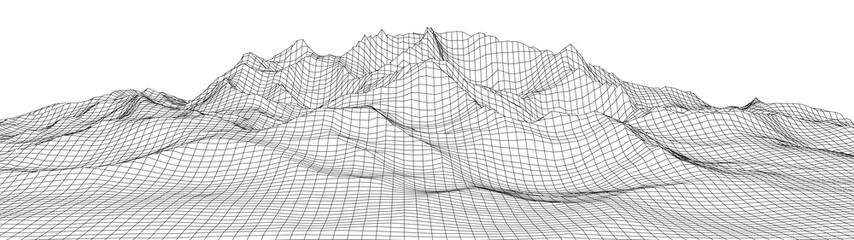
\includegraphics[width=\paperwidth]{./Unidad 2/Images/cover_bg_short}
\restoregeometry
\tableofcontents
\chapter{}
\section{Fracciones y decimales}
\subsection{Equivalencias de fracciones y decimales}
\subsection{Decimales peri\'odicos}
\subsubsection{Redondeo y truncamiento}

\section{Recta Num\'erica, Densidad y Orden}
\subsection{Fracciones en la Recta Num\'erica, Densidad y Orden}
\subsection{Decimales en la Recta Num\'erica, Densidad y Orden}
\subsection{Orden de fracciones y decimales}
\subsubsection{Orden en los n\'umeros fraccionarios}
\subsubsection{Orden en los n\'umeros decimales}

\section{Problemas con sumas y restas}
\subsection{N\'umeros con signo, recta y orden}
\subsection{Suma y resta de n\'umeros con signo}
\subsubsection{Suma de numeros con signo}
\subsubsection{Conmutatividad aditiva}
\subsubsection{Resta de n\'umeros con signo}

\section{Multiplicaci\'on con n\'umeros fraccionarios y decimales}
\subsection{Multiplicaci\'on con n\'umeros fraccionarios}
\subsection{Multiplicaci\'on con n\'umeros decimales}

\section{Divisi\'on con n\'umeros fraccionarios y decimales}

\section{\'Angulos, tri\'angulos y cuadril\'ateros}
\subsection{\'Angulos y rectas paralelas}
\subsection{Suma de los \'angulos interiores de un tri\'angulo y de un cuadril\'atero}
\subsubsection{\'Angulos de un tri\'angulo}
\subsubsection{\'Angulos de un cuadril\'atero}

\section{Tri\'angulos, cuadril\'ateros y congruencia}
\subsection{Criterios de congruencia}





\chapter{}

\section{S8 Jerarqu\'ia de operaciones y signos de agrupaci\'on}
\subsection{L1 Jerarqu\'ia de operaciones y signos de agrupaci\'on}
\subsection{Introduction}
\end{document}
